% !TEX root = /Users/royc/Google_Drive/Thesis/RoyC_Umass_Thesis.tex
\chapter{Discussion} 
\label{Disc}
\lhead{Chapter 5. \emph{Discussion}} 
%----------------------------------------------------------------------------------------
\section{Concerning the Transcriptome}
  \label{Disc:sec:Future of Dynamic long RNAs}

  Deep sequencing of transcriptomes has revolutionized biology. Previously, transcript identification and characterization involved significant labor, cost, and materials. In the mid-90's, microarray technology \citep{Schena1995a} gave us a tantalizing glimpse into how genes were expressed, but were limited to probed, and therefore known, sequences. Yet, these green and red landscapes hinted at incredible complexity---a complexity that would have to wait for technology to catch up.

  RNA-seq was made possible by incremental improvements in numerous supportive technologies. These included: 1) digital optics; 2) microscopy; 3) slide chemistry ; 4) colony PCR; and 4) nucleic-acid alignment. A HiSeq 2500 relies on all of these technologies (and others) to produce the 100M+ sequences that allow scientists to peer into the transcriptional output of a genome.

  The past five years have brought further improvements, allowing biologists to think beyond mRNAs and small RNAs. The former captured our interest for 30+ years \citep{Furuichi1975,Wei1975}, while the later has been on a run-away train since 1998 \citep{Fire1998}. Long RNAs (including lncRNAs) are now routinely analyzed by HTS. However, many biologically-trained and minded Scientists find themselves overwhelmed by the completely different methods and approaches used to tackle these biological ``big data.'' Current experimental training does not provide most with the required skills in statistics, programing, and experimental design needed to work with genome-wide data (see section \ref{Disc:subsec:Biologists need Comp Skills}). The richness of these data often results in unasked, and unanswered, testable hypothesis just sitting in public data repositories \citep{Plocik2013}.

  This discussion will focus on \textit{long RNAs} containing traditional mRNA features---a 5\textprime~m7G Cap, ligated exons, and a poly(A)+ tail. Many of these long mRNAs are extremely dynamic. So much so that until HTS and RNA-Seq, comprehensive investigation of their complexity was not possible.

  \subsection{Pervasive transcription}
    \label{Disc:subsec:Pervasive Tx}

    There are $2,598,960$ different Poker hands possible from a 52-card deck. There are $1,098,240$ different single-pair combinations, with a probability of obtaining one being almost 50\%. Compare this to a ``Royal Flush'', for which there are only 4 options, and a probability of $649,739:1$ or $1.54 * 10^{-6}$ !. It is these numbers that makes possible to play Poker for hours on end. Biology uses similar combinatorics to arrange exons into unique and rare combinations, especially in complex eukaryotic organisms. Indeed the process of splicing is closely correlated with organism complexity. The process of AS is even more closely tied to organism complexity (Figure \ref{Intro:fig:numGenesAndNumSpliced}). Accurate determination and assembly of each card (exon) that comprises a hand (transcript) is a major ``known unknown'' \citep{Rumsfeld2011} of research into long RNAs.

    The ENCODE papers from late 2012 suggested that 95\% of the genome is functional \citep{Dunham2012}, a finding that continues to be heavily debated \citep{Graur2013,Bhattacharjee2014}. \citet{Djebali2012} and focused on issues of transcription in these cell lines, as discussed in section \ref{Intro:subsec:IsoformsPerGene}, and concluded that 75\% of the genome is transcribed into RNA. Additionally, GENCODEv7 includes 9,640 manually curated lncRNA loci, some of the most novel and functionally interesting class of long RNAs \citep{Derrien2012,Pauli2011}. While ENCODE was performed using multiple human cancerous cell lines, these results support the ability of HTS to reveal transcriptional diversity.

  \subsection{A need for transcript assembly}
    \label{Disc:subsec:need for Tx assembly}

    The current state of the transcriptome assembly, a field in its relative infancy, is described in section \ref{Intro:subsec:Tx Assembly}. Current transcript assembly algorithms only provide predictions and probabilities for the existence of real molecules. Until RNA can be directly sequenced, in their entirety, and from single cells or molecular compartments, researchers will always be making compromises in annotation and quantification \citep{Ozsolak2010}. Once technology advances to the point where a transcriptome can be as accurately and quickly determined as a genome, extremely exciting research into the more subtle and nuanced complexity (e.g. what makes one twin \textit{molecularly} different from another?) of biology can be unlocked.

    What is required to improve our ability to quickly and accurately assemble transcriptomes? Simulations indicate that improvements will not come from longer read lengths \citep{Chang2014c}. These simulations also demonstrate that the accuracy of current \textit{de novo} (see section \ref{Intro:subsec:Tx Assembly}) assemblers decreases sharply with increased increase AS within the transcriptome. \citet{Engstrom2013}, who performed a systemic assessment of RNA-Seq transcript reconstruction methods concluded what is likely to be the most revolutionary step toward accurate transcriptome assembly---single pass sequencing of single transcripts. Results presented by \citep{Sharon2013}, demonstrating inherent constraints imposed by requiring RT to convert long RNAs to long cDNAs, mean that this future single-molecule sequencing will have to be of the RNA directly. This will be especially important and informative to pickup modifications such as N6-methyl-adenosine \citep{Pan2013}

  \subsection{Tissue and cell specificity}
    \label{Disc:subsec:Tissue-specific Tx expression}

    As discussed in section \ref{Intro:subsec:Alternative Splicing}, mechanisms of AS are frequently tissue-, time- and cell-specific. Landmark studies examining AS in different organ systems, from evolutionarily-distant organims, found that AS is more comparable between organs of different animals than between different organs from the \textit{same} animal \citep{Barbosa-Morais2012,Merkin2012}. \citet{Brown2014} analyzed the \flies{} transcriptome, and observed that AS could be better desribed as ``tissue-specific splicing''. Further, tissue-specific lnRNA expression has been recently reported \citep{Washietl2014}, adding to the importance of sample resolution performing transcriptome analysis.

    The concept of ``tissue-specific splicing'' brings up a subtle, but important consideration concerning AS research. The concept of AS conjures an image of dynamic post-transcription RNA processing, allowing cells to quickly respond changes in environment, programming, or stimuli. Yet, as demonstrated by the studies just mentioned, most AS is not that dynamic. In fact, the main reason much of these events are even considered \textit{alternative} is because we are comparing the transcriptomes of different tissues. Is that a fair comparison?

    By the current definition, these events are indeed \textit{alternative}, but does that label carry significance? The label of alternative communicate that RNA products of a gene can be processed into multiple ways, but if they are typically \textit{not} alternatively splicing in the local environment, does this capability matter when HTS allows analysis of very specific biological samples and time points? These questions underscore the importance of advances in transcriptme assembly keeping step with advancements in HTS technology and ever-increasing sample resolution.

  \subsection{Lingering Questions for \dscam{}}
    \label{Disc:sec:Dscam}

    What controls the stochastic and probabilistic splicing of \dscam{}? Why is it different between hemocytes and neurons? Why would hemocytes need less apparent diversity, given the range of antigen they could potentially encounter?

    Can methods such as RNACapture be used to perform more careful and targeted sequencing of \dscam{} transcripts \citep{Mercer2014}?

\section{In the haystack: piRNA Precursors}
  \label{Disc:sec:piRNA precursors}

  Chapter \ref{MolCel} describes the annotation of 467 transcripts from 214 loci. These loci account for 95\% of the total piRNAs in 14.5 dpp mice. These transcripts possesses the archetypical molecular signatures of Pol II origin, including 5\textprime~MeGpppN caps, introns, and poly(A)+ tails. Yet, RNA from these molecules appears to be rapidly consumed and processed into millions of unique small RNA (~24\textendash32 nt) species. How does the cell partition mRNAs for translation by the ribosome or cleavage and maturation into piRNAs?

  \subsection{Precursor Identity}
    \label{Disc:subsec:How are precursors generated}

    A good example to highlight why this is an issue is shown in Figure \ref{Disc:fig:wdfy3}. In testes of mice, the \textit{pi-Wdfy3} locus produces at least two different transcripts from different promoters. Virtually all piRNAs map within the bounds of the shorter isoform. The promoter that falls more 3\textprime~ within the gene is also bound by A-MYB. The more 5\textprime~ promoter, which presumably drives transcription of the longer isoform, is not bound by A-MYB. Also, in \amyb{} mutants, piRNAs from the shorter locus drastically reduced as did RNA-Seq reads. RNA-Seq reads aligning to the longer transcript did not decrease. 

    \begin{figure} % pi-Wdfy3 expresses both mRNA and piRNA precursor transcript
      \centering 
      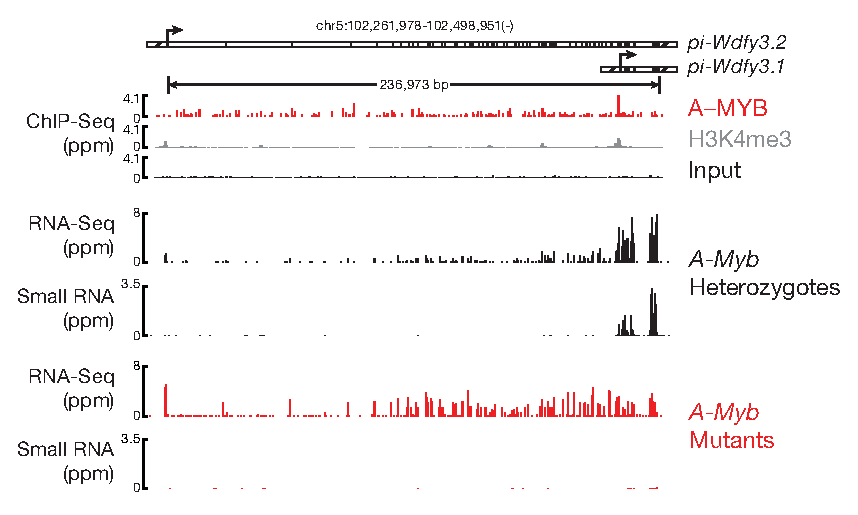
\includegraphics{Figures/Discussion/pi-wdfy3.eps}
      \caption[\wdfy{} locus expresses both mRNA and piRNA precusor form in testes]
      {\wdfy{} locus expresses both mRNA and piRNA precusor form in testes\\[0.25cm]
        The mouse genomic locus \wdfy{} expresses both a traditional mRNA form, originating from an upstream TSS, and a piRNA precursor transcript from a downstream TSS. The piRNA precursor form appears to originate from an A-MYB-bound promoter, and is expressed in \amyb{} heterzygous mice. Also smalll RNAs (piRNAs) mapping to this locus are only observed in \amyb{} heterzygous mice, and not in \amyb{} mutant mice.
        }
      \label{Disc:fig:wdfy3}
      \end{figure}

    These results indicate that A-MYB drives transcription of the shorter \textit{pi-Wdfy3} locus, but not longer transcripts, annotated elsewhere as \textit{Wdfy3}. A general phenomenon of piRNAs mapping to the 3\textprime~-UTR of mRNAs has been reported \citep{Robine2009}. How does a cell discriminate between these two transcripts and partition them for use as mRNA or processing into piRNAs?

    What determines that a seemingly mRNA-like piRNA precursor is processed into piRNAs, and not translated like crazy by Ribosomes? Recently, it was demonstrated that virtually all RNAs interact with the ribosome \citep{Ingolia2011}. This observation was later refined to state that only mRNAs display a strong ``Ribosome Release Score (RRS)'' indicative of read-frame engagement \citep{Guttman2013}. Therefore, it is not surprising that preliminary results support precursors being traversed by ribosomes (Xin Zhiguo Li, unpublished). Additional experiments and bioinformatic analysis may tease out sequence elements the assist in precursor discrimination from mRNAs by the ribosome, similar to the RRS for traditional ncRNAs.

    Beyond ribosome profiling, what are other potential experimental approaches that could be used to gain further insight into the biology of mammalian piRNA precursors?

  \subsection{Precursor Interaction}
    \label{Disc:subsec:Labeling of precursors}

      Intergenic piRNA loci share many features of traditional Pol II transcripts (Figure \ref{SeqZipMethod:fig:piRNA precusor Tx features}), with the exception of one almost half contain no introns. Visual inspection using genome browsers and the HTS datasets described in Chapter \ref{MolCel} revealed how unique these loci are from the rest of the transcriptome. Can precursor characteristics be exploited to gain further insight into their biology?

      As discussed in sections \ref{Intro:subsec:Alternative Splicing} and \ref{Intro:subsec:Splicing Code}, splice sites and SRE are recognized amidst a sea of extremely similar ``crytic'' sequences. The spliceosome is remarkably efficient at determining the correct elements to use. Also, core spliceosomal components also assist in choosing from this the overwhelming set sequences. \citet{Berg2012} identified the snRNP U1 as a key suppressor of cryptic polyadenylation site (PAS) use. This suppressor activity is in contrast to its primary role in the definition of 5\textprime~ splice sites. Perhaps a similar mechanism is acting on cryptic splice sites contained within precursor pre-mRNAs. What experiments could be used to identify precursor interacting molecules, protein and RNA both?

      Coincident with HTS development, methodology to measure genome-wide interactions have also made considerable advances \citep{Konig2011}. Methodologies to capture Protein::RNA interactions include ``HTS-CLIP'' \citep{Licatalosi2008}, ``PAR-CLIP'' \citep{Hafner2010}, and ``iCLIP'' \citep{Konig2010}. DNA::RNA interactions are measurable using ``ChIRP'' \citep{Chu2012}, RNA::RNA interactions by ``RAP'' and ``CLASH'' \citep{Engreitz2013,Helwak2014}. Some of these approaches could be applied to determining piRNA precursor transcript interacting molecules, but there are some important caveats that warrant discussion.

      Techniques mentioned above that investigate Nucleic acid::Protein require a target protein. This approach has already been done for MILI and MIWI in postnatal testes \citep{Vourekas2012}, and few additional interacting proteins are known, limiting the number of proteins to investigate. Obvious initial candidates include MitoPLD, Mvh \citep{Lasko2013} (the mouse homologue of Vasa) and numerous Tudor-related proteins \citep{Chen2011}.

      Also, genome-wide measurement of Nucleic Acid::Protein interactions typically require cross-linking \citep{Chodosh2001} using either ultra violet light, or reagents such as glutathione. This requirement is why most original reports of these techniques are performed in cell culture, due to the relative easy of exposing the sample to the cross-linking reagent. Currently, the process of piRNA biogenesis has only been reproduced in vitro using silk worm cell culture extracts \citep{Kawaoka2009,Kawaoka2011}, a system which is likely far from that of pachytene biogenesis and function in mice. Therefore, application of these techniques to mammalian piRNA pathway study would require sectioning of testes prior to cross-linking. \citep{Vourekas2012} worked around this requirement by detunicated testes and creating a cell suspension in a petri dish which was then irradiated. Another potential work-around for would be to perform these studies in mature (or \textit{maturing}) sperm. However, how much of exciting biology driven by piRNAs has already occurring once sperm have transitioned into the epididymis?

      Nucleic Acid::Nucleic acid interactions typically require a ligation step, the efficiency of which is typically very low \citep{Helwak2014}. Additionally, the ``ChIRP'' protocol is done in crude cell extract, where RNAse H is a concern when using DNA probes to investigate pull down or query RNA. Given that precursor transcripts seem to be rapidly processed (section \ref{SeqZipMethod:sec:piRNA precursor by SeqZip}), these methods may require prior enrichment, perhaps using RNACapture \citep{Mercer2014}, as discussed for \dscam{} above (section \ref{Disc:sec:Dscam}. Given recent developments into the CRISPR/CAS9 system for genome-editing \citep{Sander2014}, the ``CLASH'' approach to looking at RNA::RNA interactions for precursor transcripts is attractive. The requirement for a tagged protein, in this case an PIWI protein like MILI or MIWI, is no longer as large a barrier.

      These approaches could also be used for to analyze mature or developing sperm as they move through the seminiferous tubules and into the epididymis. It is in epididymis where sperm mature and piRNAs are known to be ``sequenceable'' (at least in humans) \citep{Jones1999,Li2012a}.

      As the methods and experimental techniques discussed above evolve and become more robust, applications to the biogenesis of piRNA biology will be many. Increased resolution of timepoints, proteins, and species examined will help create a comprehensive purpose for piRNA in the maintence of mammalian male fertility.

  \subsection{Precursor Location}
    \label{Disc:subsec:Imaging of precursors}

    Determining genome-wide protein and nucleic acid interactors with piRNA precursor transcripts would produce valuable datasets. A major drawback of all the methods and approaches discussed above is that they do not maintain the anatomical and cellular location of transcripts. Localization of RNA has been important for decades \citep{Rebagliati1985}, and was recently shown is a large screen in \flies{} embryos to be the rule rather than the exception \citep{Lecuyer2007}.

    The most important question for mammalian \textit{pachytene} piRNAs is \textit{What are they doing?}. We know that they are essential for the health of the species, as discussed in section \ref{MolCel:sec:Introduction}, and piRNA-pathway mutants are sterile. What could these small RNAs, with complementarity to nothing but themselves, be doing? 

    The cellular location of precursor piRNA transcript processing is not known. The most accepted hypothesis is that precursor transcripts are processed into mature piRNAs with machinery tethered to chromatoid bodies \citep{Meikar2011,Meikar2014} or another structure similar to Drosophila Nuage near the mitochondrial cement. Knowledge of \textit{where} mature piRNAs are generated would provide clues into larger mechanist details of their biogenesis. 

    I can think of two broadly different ways in which we could pinpoint the physical location of mature piRNA generation. The first is to chemically label, in some manner, primary piRNA transcripts. The label would need to 1) not interfere with processing and 2) be durable to later methods used to analyze the presence or absence of the modification. A second way to identify the location of mature piRNA processing would be to actually observe, through in vivo \hyperref[hd:abrevs]{FISH}, the various products and by-products of biogenesis. In this particular approach, SeqZip maybe useful.

    %SeqZip accurately reports on the presence of multiple, distant sequences contained in the same RNA molecule (see Chapters \ref{SeqZipPaper} and \ref{SeqZipMethod}). Yet I was not able to observe ligation products templated off some of the most highly-expressed precursor transcripts (see section \ref{Disc:sec:piRNA precursors}. We hypothesize that the most likely explanation for being unable to observe ligation products for these transcripts, but successfully observing those for a very long, but lowly expressed gene \textit{Dst}, suggests that precursor transcripts are rapidly processed into mature piRNAs. What if this is not the case if we could hybridize ligamers to precursor transcripts in vivo? Put another way \textemdash What if the steady-state amount of precursor transcript is very low due to rapid processing, but when visualized in real time, the transcripts are of sufficient abundance for FISH? Ligamers could be engineered to contain different combinations of fluorescent dyes, and the proximity and intensity of the signal could be used to infer precursor transcripts. Importantly, this approach could distinguish long, continuous precursor transcripts from processing intermediates and mature piRNAs.

    Improvements in \textit{in vitro} FISH experiments allow for discrimination of isoforms resulting from alternative splicing \citep{Lee2014}. Robust FISH-type experiments could be used to investigate cellular and anatomical locations of  precursor transcript processing. The SeqZip methodology could even be used in this regard (see section \ref{Disc:subsubsec:SeqZip and Single-Molecule FISH}). 

    Beyond FISH, and using the previously mentioned CRISPR/CAS9 systems, traditional MS2 loop sequences could be introduced into piRNA-generating genes, similar to experiments performed in the the Singer lab \citep{Park2014}. Mice expressing precursors contaning MS2 loops could be crossed with those containing MS2 Bacteriophage capsid protein fused to GFP (MCP-GFP). Using this system precursors could potentially be visualized in real time or at least in real locations.

  \subsection{Precursor Sequencing}
    \label{Disc:subsec:Sequencing of Precursors}

    Very recently, methods demonstrating sequencing \textit{in situ} have been published \citep{Ke2013,Lee2014a}. These methods represent a major improvement over single-cell sequencing approaches discussed in section \ref{Intro:subsec:Types of HTS} in that they maintain the cellular location of the sequenced RNAs. Building upon the principles of FISH, sequencing allows for novel sequence discovery, and multiplex investigation (FISH allows for a maximum of 4--5 transcripts to be examined at once). Could \textit{in situ} sequencing be used to learn more about piRNA precursor biology?

    FISSEQ, reported by \citet{Lee2014a}, replies on rolling circle amplification to create a 3D grid of highly concentrated DNA (``nanoballs''), originating from a single RNA/cDNA. SOLiD sequencing is used to determine 27--30 bases from each nanoball, followed by assignment of that sequence to a grid location thus joining sequence and location. Read lengths for FISSEQ would make it difficult to distinguish a mature piRNA from a precursor, and an experimental scheme, perhaps exploiting the methylation of mature piRNAs, would have to be used to ensure the sequencing of precursor or intermediate molecules.


\section{Future of RNA-templated DNA-to-DNA ligation}
  \label{Disc:sec:SeqZip Improvements}

  The SeqZip methodology as developed and described in Chapters \ref{SeqZipPaper} and \ref{SeqZipMethod} works adequately and robustly for characterization of relaLee2014tively simple (\cd{}) to extremely complex (\dscam{}) genes. However, there is still substantial room for method optimization. Two obvious areas of improvement include the reduction of ligation time and NTL product formation. The improvements and modifications discussed below should assist in achieving these two (among other) goals.

  \subsection{An optimized SeqZip examination of Coordinated splicing}
    \label{Disc:subsec: Ideal SeqZip exp. to look for Coordination}

    If I could go back in time 4 years and still possess the knowledge and abilities that I do now, I would have approached a genome-wide study of coordination in splicing using SeqZip much differently. First, I would have focused on alternative first exon (or promoter, or TSS) and potential coordination with downstream cassette exons. I would have mined newly-generated RNA-Seq data \citep{Wang2008, Pan2008} for alternative first exons and cassette exons of sufficient expression. Then, I would have used my automated ligamer design software (see Appendix \ref{Appendix:AutoMatedLigamerAssembly}), to create a database of the required ligamers. As this would require at least 3 ligamers per event, with very little duplicated use of ligamers, the number of ligamers would make standard synthesis, even using 384-well plates, impossible. Therefore, I would have pursued printing the ligamers on a custom microarray, and cleaved them into solution, similar to products offered by \href{http://www.nimblegen.com/}{Nimblogen}. These ligamers would be barcoded and priming sequences included such that short (50nt) paired-end reads could reliably identify the templated first and cassette exons. Using this pool of ligamers, I would have performed the SeqZip assay, including a barcoding scheme to quantify the number of ligation events per {alt first exon::cassette exon} pair. Also, the libraries would have been amplified via digital PCR allowing me to check for PCR jackpots \citep{Shiroguchi2012a}. Finally, the data would be aligned against a reference of all \{alt first exon::cassette exon\} pairs, and any potential coordination determined.

    If I could have done the experiment designed above, I feel the full potential and utility of the SeqZip method could have been realized and generated new and valuable knowledge for the field of gene expression.

  \subsection{LNA-containing ligamers and T39A Rnl2}
    \label{Disc:subsec:LNA-Containing ligamers and T39A Rnk2}

    The use of an RNA-base on the 5\textprime~side of the nick encourages a C3\textprime~\textit{endo} sugar pucker for the base, placing the 3\textprime~OH in an apical orientation relative to the the AMP leaving group (Figure \ref{Disc:fig:Rnl2 and suger pucker}) \citep{Nandakumar2006}.

    \begin{figure} % Rnl2 Suger Pucker
      \centering 
      \includegraphics{Figures/Discussion/Rnl2_and_suger_pucker.eps}
      \caption[Suger pucker in Rnl2 structures]
      {Suger pucker in Rnl2 structures \\[0.25cm]
        Using two different nucleic acid substrate combinations crystallized with Rnl2, \citet{Nandakumar2006} demonstrates the effect of 3\textprime~and 2\textprime~ identify of the base at the 5\textprime~side of the nick: Left) The crystal structure (PDB: 2HVS), containing a 2\textprime~ position deoxy residue, displays a DNA-like C2\textprime~\textit{endo} sugar pucker. In contrast to Right) where the crystal structure (2HVR) contains a 2\textprime~ hydroxyl and displays an RNA-like C3\textprime~\textit{endo} sugar pucker.
        }
        \label{Disc:fig:Rnl2 and suger pucker}
        \end{figure}

    With lowered costs of oligo synthesis, incorporation of 2\textprime~OMe at the penultimate and ultimate bases of the 5\textprime~nick ligamers should greatly increase ligaiton efficiency, as these are the primary substrate-specificity determinants of Rnl2 \citep{Nandakumar2004a, Nandakumar2006}.

    Interestingly, \citet{Nandakumar2004a} demonstrated that the ribosome at the penultimate position, evidenced by a 50-fold reduction in turnover number for 2\textprime~H substitutions at this position, compared to full activity for 2\textprime~OMe. \citet{Nandakumar2006} (Figure \ref{Disc:fig:Rnl2 and suger pucker} shows that Threonine 39 (T39) hydrogen bonds with both the 2\textprime~OMe and 3\textprime~O of the penultimate suger. A T39A mutation did not phenocopy the 2\textprime~H substitution on the penultimate suger, indicating that suger pucker is the structural constraint on ligation efficiency. These results indicate that a T39A mutant of Rnl2 may demonstrate increased RNA-templated DNA:DNA ligation efficiency, as it would have one less molecular requirement for RNA.

    Future versions of the SeqZip assay could use a combination of LNA modified bases \citep{You2006} at either the penultimate or terminal residues on the 5\textprime~side of the nick in order to increase 1) specificity, and 2) enzyme efficiency. The combination of these modifications in the ligamers could be combined with a T39A mutant form of Rnl2 for a potentially greatly enhanced ligation rate.

  \subsection{Thermostable Ligases}
    \label{Disc:subsec:Thermostable Ligases}

    The use of LNA-containing brings up issues involving off-target hybridization. Future iterations of the SeqZip methodology could use directed protein evolution of Rnl2 \citep{Stemmer1994, Romero2009a} to develop a thermostable variant of Rnl2, similar to variations of DNA ligase that have been used for years \citep{Barany1991}. Use of LNAs and elevated ligation temperatures could alviate off-target hybridization events reducing both nonproductive hybridization and non-templated ligation events. This would also allow for use of reduced overall ligamer concentrations, in line with the optimal SeqZip experiment described in section \ref{Disc:subsec: Ideal SeqZip exp. to look for Coordination} and synthesis on microarrays.

  \subsection{Other SeqZip Applications}
    \label{Disc:subsec:Future Uses of SeqZip}

    SeqZip can be used to many different forms of RNA sequence characterization. An incomplete illustration of these applications is shown in Figure \ref{Disc:fig: Panel of SeqZip Applications}. The three novel applications are discussed below:

    \begin{figure} % SeqZip uses Panel
      \centering 
      \includegraphics{Figures/Discussion/SeqZipUses.eps}
      \caption[Proposed uses of the SeqZip methodology]
      {Proposed uses of the SeqZip methodology \\[0.25cm]
        Shown here are general applications of the SeqZip method to profiling RNA sequences. Top row examples are substantiated by experiements described on Chapters \ref{SeqZipPaper} and \ref{SeqZipMethod}, the middle and lower rows are hypothetical but logical extensions of the method.
        }
      \label{Disc:fig: Panel of SeqZip Applications}
      \end{figure}

    \subsubsection{Multi-site SNP detection}
      \label{Disc:subsubsec: Multi-site SNP Detection}

      The concept of connectivity in sequence can be applied not only to exons, or long stretches of RNA, but even to single-nucleotides, as in SNPs. SeqZip could be used to profile potential SNPs contained within the same transcript, and therefore within the same allele (Figure \ref{Disc:fig: Panel of SeqZip Applications}). For maximal benefit and specifity, care should be taken as to where the variant bases are placed in the ligamers, respective to the 5\textprime~ or 3\textprime~ side of the nick to be ligated. \citet{Chauleau2013b} have demonstrated the importance of proper base pairing at the 3\textprime~OH side of the nick. 

    \subsubsection{SeqZip and single-molecule multi-site FISH}
      \label{Disc:subsubsec:SeqZip and Single-Molecule FISH}

      \begin{figure} % Multi-site Fish using SeqZip
        \centering 
        \includegraphics{Figures/Discussion/MultiSiteFish.eps}
        \caption[Multi-Site smFISH using flourophore-containg ligamers]
        {Multi-Site smFISH using flourophore-containg ligamers \\[0.25cm]
          The simplest form of a multi-site FISH SeqZip experiment. Five ligamers are used, with two hybridizing to the beginning and end of a target sequence of RNA (e.g. and exon), and having unique fluorescent labels (Cy3 and Cy5 in this case). The use of the third ligamer, containing an addressable barcode is used to report on these two ligamers hybridizing to the same RNA. Use of flanking ligamers allows for amplification and additional analysis and trouble shooting, if desired.
          }
        \label{Disc:fig:MultiSite FISH using SeqZip}
        \end{figure}

      A logical extension of the multi-site SNP detection application described above is the use of SeqZip in multi-site FISH probes. Represented in Figure \ref{Disc:fig:MultiSite FISH using SeqZip} is the most simplistic form of this application. Advances in FISH, microscopy, flourscent moieties, and image processing are making this type of experiment much more approachable. A multi-site FISH SeqZip experiment could be used to ask some of the questions described in section \ref{Disc:subsec:Imaging of precursors}, including precursor integrity and location, without the need for downstream processing.

    \subsubsection{Introduction of destruction sequences}
      \label{Disc:subsubsec:Intro of Desctruction Sequences}

      Introduction of unique sequences into a ligation product is one of the most useful aspects of the SeqZip method. In addition to the other uses proposed (barcoding, sites of priming, sequence diversity, etc), the sequences introduced could also be used to \textit{eliminate} ligation products, through restriction enzymes or pulled out via selective hybridization, similar to selective removal of ribosomal RNA sequences during HTS library preparation \citep{Chen2011a}.

    \subsubsection{Re-purposing the SOLiD Platform}
      \label{Disc:subsubsec:SOLiD Platform for SeqZip}

      Custom sequences within ligamers could also be used to generalize exon identity. Put another way, ligamers representing the first exon of a message could be given a specific barcode, second exons another barcode, and so on. Then, using a sequencing platform such as SOLiD and custom hybridization/sequencing oligos, florescent signal would report not the sequence, but the identity of the ligamer, and by proxy the numeric ID of the exon within the target message. A few rounds of traditional sequencing could identify the mRNA from each spot, and a simplistic scheme of exon arrangement for a complete mRNA could be interpreted from the ligation product. Of course this would require major optimization to the SeqZip method, heavy bioinformatic transformation of a given transcriptome annotation, transcriptome-wide design and synthesis of ligamers, and customization of the SOLiD platform including ligation chemistry. But it would be extremely useful and informative for complete and routine transcriptome quantification.

\section{Final Thoughts}
  \label{Disc:sec:Final Thoughts}

  This thesis has introduced the complexity, purpose, potential, and challenges of transcriptome study. There is no comparison between these issues with that of the DNA genome. The next period of biomedical knowledge will be heralded by advances in transcriptome analysis. This section discusses how scientists need to grow with technology.

  \subsection{Science vs. Engineering}
    \label{Disc:subsec:Science and Engineering}

    \begin{quote}
      \itshape 
      \singlespacing
        “There is a general attitude among the scientific community that science is superior to engineering.” - \citep{Macilwain2010}

      “Science is about what is; engineering is about what can be. Engineers are dedicated to solving problems and creating new, useful, and efficient things.“ - Niel Armstrong
      \end{quote}

    A common schism between technically-oriented individuals is whether or not they identify themselves as an engineer or a scientist. The first quote, from an article published in Nature, communicates a clear bias in academic circles of the importance of the \textit{why} over the \textit{how}. In essence, how one prioritizes these questions categorizes individuals as scientists (why is important) or engineers (how is more important). The second quote, from the first man to walk on the Moon, Neil Armstrong, highlights what motivates a self described ``engineer'' and ``geek.'' How does a graduate system--- training PhDs for careers in life science--educate individuals who fall into these two fundamentally different belief systems?

    Not well. When searching for a lab I told professors that I wanted to work on a technology development project. A typical response was, ``That's not what we do here.'' As someone who is more interested in the ``how'' over the ``why,'' this began a brief period when I thought I had made the wrong choice leaving industry and going back to graduate school. What was the basis for this aversion to technology development? The same article in Nature states that this feeling toward engineering may be attributed...

    \begin{quote} 
      \itshape 
      \singlespacing
      ...partly to a ``linear'' model of innovation, which holds that scientific discovery leads to technology, which in turn leads to human betterment. This model is as firmly entrenched in policy-makers' minds as it is intellectually discredited. As any engineer will tell you, innovations, such as aviation and the steam engine, commonly precede scientific understanding of how things work.
      \end{quote} 

    If policy-makers value basic discovery over technological application, perhaps this explains why many of my professors tried to steer me away from a technology development project.

    In spite of policy-makers and my professors holding the viewpoint that discovery precedes technology, some of the most notable breakthrough scientific discoveries, including many made by Nobel Laureates, demonstrate a clear integration of both the scientific method and technological application. For example, the 2007 award in Physiology and Medicine was given for ``discoveries of principles for introducing specific gene modifications in mice by the use of embryonic stem cells."  By combining these principle discoveries, an indispensable technique in modern genetics was created---gene targeting. The feeling of which is more important, the principle discoveries or the application thereof, is likely what separates a scientist from an engineer.

    The importance of technology to the advancement of science in general is not limited to anecdotes resulting in a Nobel prize. A quick scan of the most \href{http://www.pnas.org/reports/most-cited}{highly-cited} papers in the journal PNAS reveals that the top 13, indeed \textit{all} 13, are about a novel methodology or technique. Sequencing of DNA, microarray analysis, tetracycline-inducible promoters, recombinant adenovirus, and site-specific mutagenesis are just a handful of the tools on the list. This effect can also be seen in \href{http://simplystatistics.org/2014/04/07/writing-good-software-can-have-more-impact-than-publishing-in-high-impact-journals-for-genomic-statisticians/}{computation biology}, with transformative algorithms, such as BLAT \citep{Altschul1990} and Bowtie \citep{Langmead2009} attain citations well beyond a typical paper in their journal of publication and far more than most primary research articles.    

    The growth of big datasets is forcing all in biomedical research to think like an Engineer. At least two major concerns require immediate attention: How to store the data and how to analyze it?

  \subsection{The Data Deluge}
    \label{Disc:subsec:Dealing with Data Deluge}

    \begin{quote}
      \itshape
      \singlespacing
      The HiSeq X Ten is sold as a set of 10 or more ultra-high throughput sequencing systems, each generating up to 1.8 terabases (Tb) of sequencing data in less than three days or up to 600 gigabases (Gb) per day, per system, providing the throughput to sequence tens of thousands of high-quality, high-coverage genomes per year. ---\href{http://bit.ly/PZpegZ}{Illumina Press Release}
      \end{quote}

    In a world where the HiSeq X, described above, is a reality, biomedical researchers need to change how they approach every aspect of data analysis. This includes storage, processing, and visualization. Evidence is mounting that replicates, not depth, aid in differential gene expression \citep{Liu2014}, which will compound the problem of using many types of very similar data and files, seperation and tracking of which will be essential.

    How do we work with all this data? Systems need to be in place to track the necessary sample meta-data, analysis and modifications to data performed, and all aid in eventual public posting and sharing of HTS data. Labrotory information management systems and Electronic lab notebooks (ELNs) must be implemented in academic labs partipating in copious amounts of HTS data.

    Once these systems are in place, the ability to navigate, via genome browsers \citep{Zweig2008,Robinson2011}, will be of critical importance to allow other members of the lab to reuse valuable datasets. Recent changes to the way aligned genomic data is stored and added to UCSC genome browsers represents a critical improvement to past methods \citep{Raney2013}. Finally, efforts such as the Galaxy project  will define how most academic labs perform ``routine'' HTS analysis in future \citep{Blankenberg2010}.

  \subsection{Biologists need Computation Biological Skills}
    \label{Disc:subsec:Biologists need Comp Skills}

    Just 10 years ago, Graduate students and PhDs in the fields of Molecular Biology or Biochemistry need not venture far from data analysis within Excel or perhaps a statistical program with an advanced graphical interface (examples include Prism or Graphpad). Software knowledge that stops at these tools and the rest of the Microsoft Office suite of tools is no longer enough to generate big strides in Biomedical research.

    Working with tens of even hundreds of lines of data within a spreadsheet is manageable and computers from 20 years ago had more then enough computing power to process the data. Yet, this type of data is longer then endpoint of most cutting edge projects. Many students and post docs often find that they are unable to analyze the data generated from months or years of tireless bench work. Faced with learning what is effectively a collection of new languages and awash in a sea of acronyms (LINUX, BASH, GNU, PERL, R) they reach out for help from a ``Bioinformatics person.'' Perhaps the relationship and interaction with this personal is productive, leading to a collaboration and exciting new knowledge. Sometimes it isn't, and the bench scientist shifts into one of three modes: 1) Wait; 2) Find another bioinformatic-minded collaborator; or 3) collect more data.

\begin{table} % Changes at the computer for Molecular biogists
  \caption[Changing computational tools for Molecular Biologists] 
    {
     Changing computational tools for Molecular Biologists
     }
   \label{Disc:tab:Comp tools for Molecular Biology}
   \footnotesize
\begin{tabular}{p{6cm}|p{8cm}}

\textbf{What is Used}            & \textbf{What Should be Used}                \\ \hline 
Word                             & Plain Text                                  \\ \hline 
Hand-inserted Citations          & Citation-management Software (e.g. Papers ) \\ \hline 
Paper Notebooks                  & Evernote or Commercial ELNs                 \\ \hline 
Excel for Data Storage                & Relational Databases (i.e. MySQL)           \\ \hline 
Excel for Data Analysis               & R or MatLab                                           \\ \hline 
Local Code development \& backup & Online Code development (GitHub)            \\ \hline 
\end{tabular}



   \end{table}

    In my experience, the most often chosen mode is ``wait.'' This is also the most damaging, as it delays the progress of one's work, and the advancement of science in general. Personally, I did not want to fall into this mode, and once the multiplex study described in section \ref{SeqZipMethod:sec:Multiplex Gene Study} reached a point where I had millions of sequencing reads, but I could not find anyone to help me analyze the data, that I decided to educate myself on the basic principles of Linux, the command line, and analysis of HTS data.

    A Biologically-train individual who posses the knowledge of analysis of HTS datasets is an extremely powerful and empowering situation. This was recently commucated in \citet{Plocik2013}:

    \begin{quote} % Polick2013 Quote about insight without a Pipette
      \itshape 
      Such exercises will empower students to explore and assess the quantitative data published in the manuscripts that they read, which can no longer be assessed at a glance like the qualitative gel-based results on which molecular biology was founded. Ultimately, it will be equally important to know how to write code as it is to pipette. - \citep{Plocik2013}
      \singlespacing
      \end{quote}

    The fact is that no one will care about a project as much as the Graduate student or PostDoc who is the main project driver. Learning and training of computational skills bent on analyzing large datasets should be central to the education in Biomedical sciences in the future.

\cleardoublepage